\documentclass[11pt,a4paper]{article}

\usepackage[a4paper, portrait, margin=1.1in]{geometry}
\usepackage[dvipsnames]{xcolor}
\usepackage[linktoc=none]{hyperref}
\hypersetup{
	colorlinks=true,
	linkcolor=blue,
	filecolor=magenta,      
	urlcolor=blue,
}

\usepackage{listings}
\usepackage{float}
\usepackage{graphicx}
\usepackage[justification=centering]{caption}
\usepackage{wrapfig}
\usepackage{amsmath}

\renewcommand{\contentsname}{Indice}

\definecolor{anti-flashwhite}{rgb}{0.95, 0.95, 0.96}

\begin{document}

\begin{center}
	\Large\textbf{Analisi delle Prestazioni dei Supercomputer}\\
	\vspace{0.2cm}
	\large{Progetto per il corso di Statistica del Prof. Marco Romito}\\
	\vspace{0.5cm}
	\large\textit{Rambod Rahmani}\\
	\vspace{0.2cm}
	\scriptsize{Corso di Laurea Magistrale in\\Artificial Intelligence and
	Data Engineering}\\
	\vspace{0.5cm}
	\normalsize{22 Novembre 2020}
\end{center}

\tableofcontents

\section{Introduzione}
Lo scopo della presente analisi \`e quello di costruire un modello di
regressione lineare multivariata per poter prevedere le prestazioni di un
Supercomputer a partire dalle specifiche delle sue caratteristiche hardware. A
partire dalla tabella dei dati, tramite l’utilizzo di R, sono stati valutati due
modelli diregressione. In particolare, uno di regressione lineare e uno di tipo
non lineare.\\
\\
Per quanto riguarda il contesto applicativo ipotizzato, esistono due benchmarks
essenziali che vengono usati per valutare le prestazioni di questo tipo di
calcolatori, il LINPACK benchmark (una misura delle prestazioni computazionali
per operazioni in virgola mobile) e il HPCG benchmark (a complemento del
LINPACK, valuta le prestazioni dei sotto sistemi del calcolatore). I costruttori
di tali computer forniscono di solito il parametro teorico (calcolato su carta)
chiamato \textbf{Rpeak} che indica le prestazioni massime teoriche. Dato che per
eseguire un test LINPACK \`e necessario calibrare ben oltre $18$ parametri,
sarebbe interessante poter stimare il valore di \textbf{Rmax} (prestazioni
raggiunte nel LINPACK test) tramite un modello statistico.

\section{Dati}
La tabella dei dati \`e stata scaricata dal sito dell'organizzazione
\textbf{TOP500}. La TOP500 mantiene una graduatoria, ordinata secondo le loro
prestazioni, dei Supercomputer attualmente installati e in funzione. Tale
graduatoria viene aggiornata con cadenza semestrale.\\
\textbf{Link di download diretto:} \url{https://www.top500.org/lists/top500/2020/11/download/TOP500_202011.xlsx}\\
\begin{figure}[h]
	\vspace{-1cm}
	\begin{minipage}{.3\textwidth}
		\textbf{Credenziali di accesso:}
	\end{minipage}
	\begin{minipage}{0.7\textwidth} 
		\begin{lstlisting}[language=bash,tabsize=2,backgroundcolor=\color{Goldenrod}]
		Login: rambodrahmani@yahoo.it
		Password: GCgFH6yuZYFMeCr
		\end{lstlisting}
	\end{minipage}
	\vspace{-1cm}
\end{figure}
\subsection{Contenuto della tabella}
La tabella dei dati contiene $37$ colonne per un totale di $500$ osservazioni.
Per la presente analisi ho utilizzato le seguenti colonne:
\begin{itemize}
	\setlength\itemsep{0mm}
	\item \textbf{Total Cores}: numero totale di cores;
	\item \textbf{Accelerator/Co-Processor Cores}: numero totale di
		cores del co-processore;
	\item \textbf{Rmax [TFlop/s]}: massime prestazioni raggiunte nel
		benchmark LINPACK;
	\item \textbf{Rpeak [TFlop/s]}: massime prestazioni teoriche;
	\item \textbf{HPCG [TFlop/s]}: massime prestazioni raggiunte nel
		benchmark HPCG (High Performance Conjugate Gradient);
	\item \textbf{Power [kW]}: potenza consumata;
	\item \textbf{Processor Speed [MHz]}: velocit\`a processore;
	\item \textbf{Cores per Socket}: numero di cores per socket.
\end{itemize}
\subsection{Importazione e pulizia}
Sui dati, non \`e stata effettuata alcuna operazione precedente la loro
importazione in R. Il file originale, in formato \texttt{.xlsx}, \`e stato
per\`o convertito in \texttt{.csv} per facilitare l'importazione.\\
Prima di iniziare l'analisi, ho rimosso le colonne che ritengo che non
influenzano le prestazioni di un Supercomputer ("Name", "Manufacturer",
"Country", "Year" ecc\dots), mentre come fattore di
uscita per la predizione utilizzer\`o il valore della colonna "Rmax".\\
Nelle colonne rimanenti, ci sono $351$ valori mancanti in
"Accelerator/Co-Processor Cores", $426$ in "HPCG [TFlop/s]" e $310$ in
"Power [kW]". Dato che il numero di valori mancanti \`e elevato rispetto al
totale delle $500$ osservazioni, le suddette colonne sono state eliminate.
\begin{wrapfigure}{l}{1\textwidth}
	\vspace{-0.5cm}
	\centering
	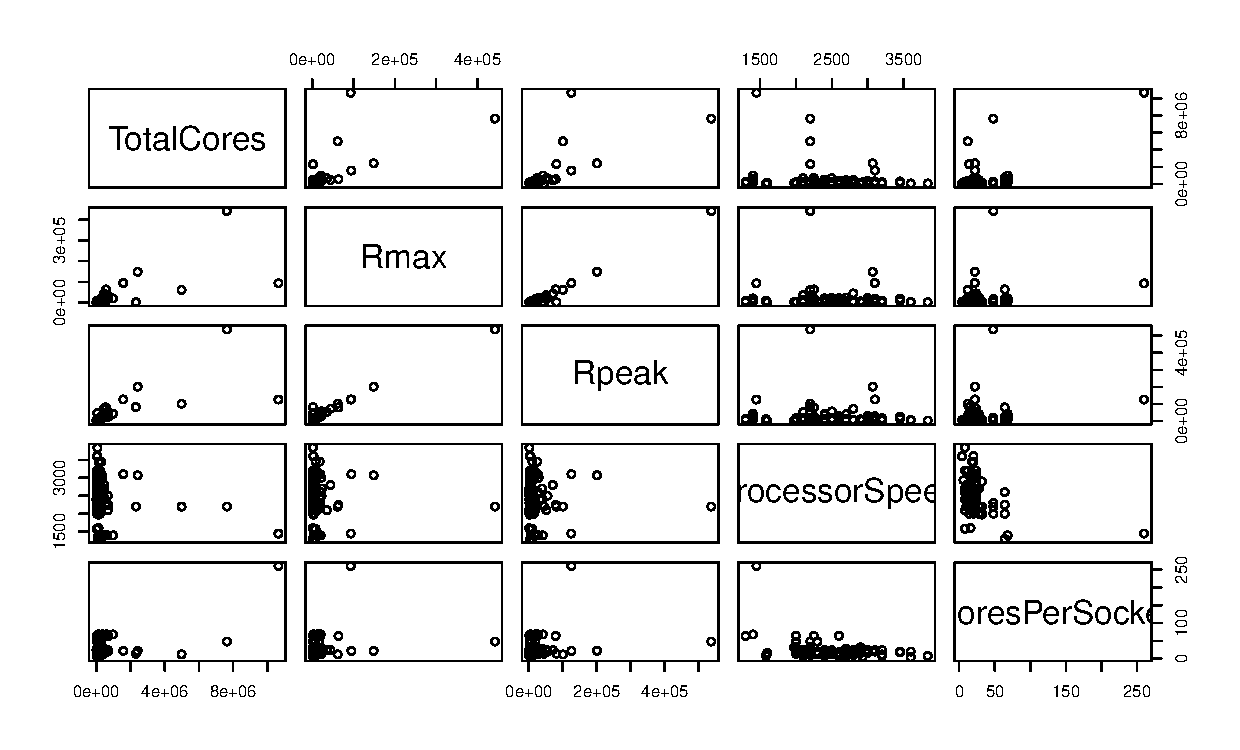
\includegraphics[scale=0.7]{imgs/plot(data).pdf}
	\vspace{-0.4cm}
	\caption{Diagramma di dispersione}
\end{wrapfigure}
\clearpage
\subsection{Esplorazione e comprensione dei dati}
\begin{wrapfigure}{r}{0.4\textwidth}
	\vspace{-1.3cm}
	\centering
	\caption{Matrice di dispersione}
	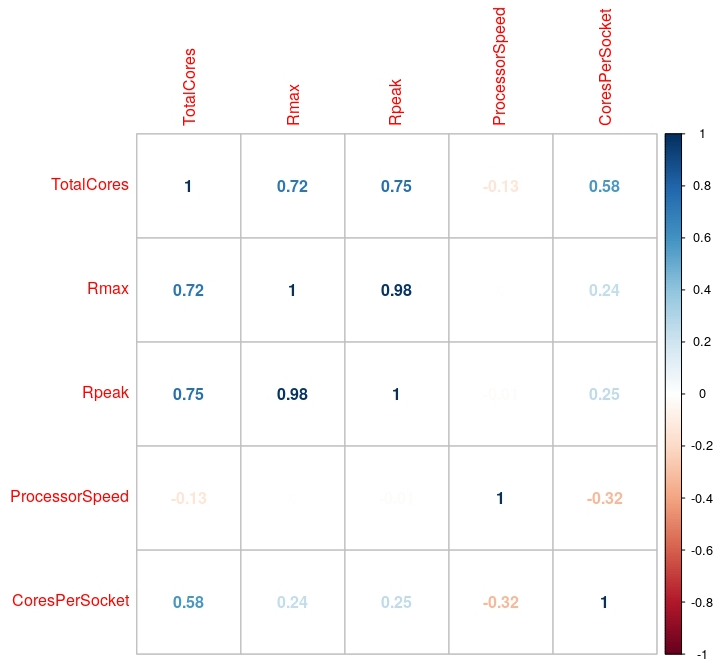
\includegraphics[scale=0.39]{imgs/cor_mat.jpeg}
	\vspace{-1.0cm}
\end{wrapfigure}
Il primo approcio esplorativo dei dati \`e stato di tipo grafico: nonostante si
possa palesemente vedere una forte correlazione tra il fattore di uscita
\textbf{Rmax} e i fattori \textbf{TotalCores} e \textbf{Rpeak}, ho preferito
iniziare con un modello di regressione lineare multipla usando \textbf{Rmax}
come output e tutte le altre variabili come predittori. Ho poi proceduto con
l'eliminazione dei fattori valutando per ogni modello ottenuto i seguenti
valori:
\begin{itemize}
	\setlength\itemsep{0mm}
	\item $\boldsymbol{R^2}$: Proporzione di Varianza Spiegata dal Modello;
	\item $\boldsymbol{R^2_{Adj}}$: Proporzione di Varianza Spiegata dal
		Modello corretto;
	\item \textbf{p-value} globale e dei singoli coefficienti.
\end{itemize}

\section{Analisi}
\subsection{Modello di Regressione Lineare}
Come primo passo, ho costruito $4$ differenti modelli di regressione lineare
valutando di volta in volta il valore di $\boldsymbol{R^2}$,
$\boldsymbol{R^2_{Adj}}$, \textbf{p-value}. Si pu\`o osservare un netto calo di
entrambi i grafici tra i punti di ascissa $3$ e $4$: dunque la terza versione
\`e la migliore delle quattro regressioni effettuate.
\begin{figure}[h]
	\hspace{-2.15cm}
	\begin{minipage}{.6\textwidth} 
		\begin{lstlisting}[language=bash,basicstyle=\tiny,tabsize=2,frame = single]
> summary(lm)

Call:
lm(formula = Rmax ~ Rpeak + TotalCores, data = data)

Residuals:
   Min     1Q Median     3Q    Max 
-59167    -74    478   1132  23307 

Coefficients:
              Estimate Std. Error t value Pr(>|t|)    
(Intercept) -1.101e+03  1.804e+02  -6.103 2.09e-09 ***
Rpeak        8.012e-01  9.450e-03  84.782  < 2e-16 ***
TotalCores  -1.392e-03  4.091e-04  -3.401 0.000724 ***
---
Signif. codes:  0 ‘***’ 0.001 ‘**’ 0.01 ‘*’ 0.05 ‘.’ 0.1 ‘ ’ 1

Residual standard error: 3889 on 497 degrees of freedom
Multiple R-squared:  0.9691,	Adjusted R-squared:  0.969 
F-statistic:  7800 on 2 and 497 DF,  p-value: < 2.2e-16
		\end{lstlisting}
	\end{minipage}
	\begin{minipage}{0.5\textwidth} 
		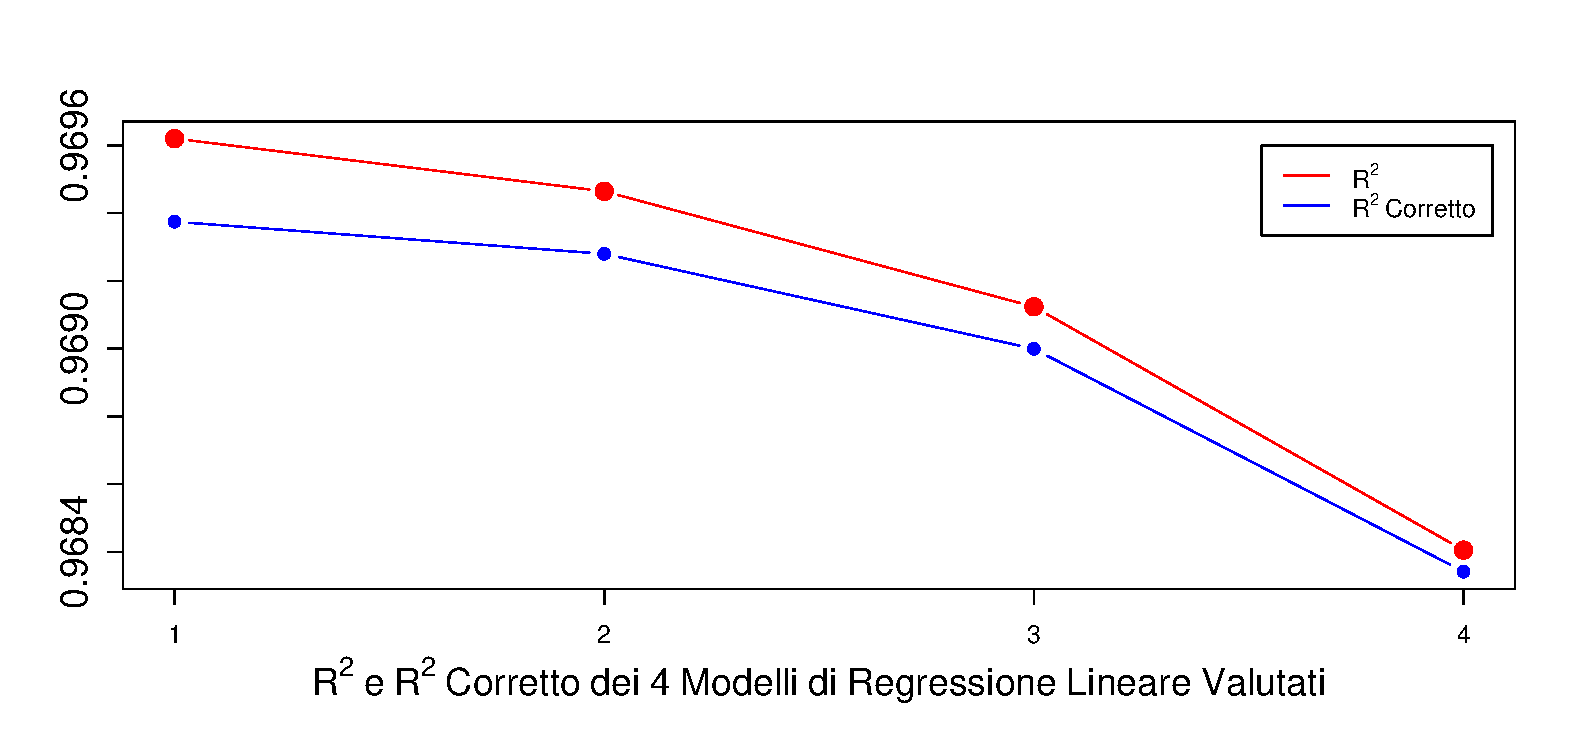
\includegraphics[scale=.4]{imgs/r_squared.pdf}
	\end{minipage}
\end{figure}
Con una proporzione di varianza spiegata dal modello maggiore del $96\%$ e con
dei p-value quasi nulli (sia per quanto riguarda i singoli coefficienti che
quello globale), possiamo concludere che il modello di regressione che abbiamo
ottenuto cattura buona parte del problema ed \`e statisticamente significativo.
\subsubsection{Analisi dei Residui}
Soddisfatto del modello ho proceduto con l'analisi dei residui. Dal diagramma di
dispersione, dall'istogramma, dal QQ\_plot e dai risultati ottenuti dal 
Test di Shapiro-Wilk \`e evidente che la distribuzione dei residui \`e ben
lontana dall'essere la Gaussiana che cerchiamo:
\clearpage
\begin{figure}[H]
	\vspace{-1cm}
	\hspace{-1.5cm}
	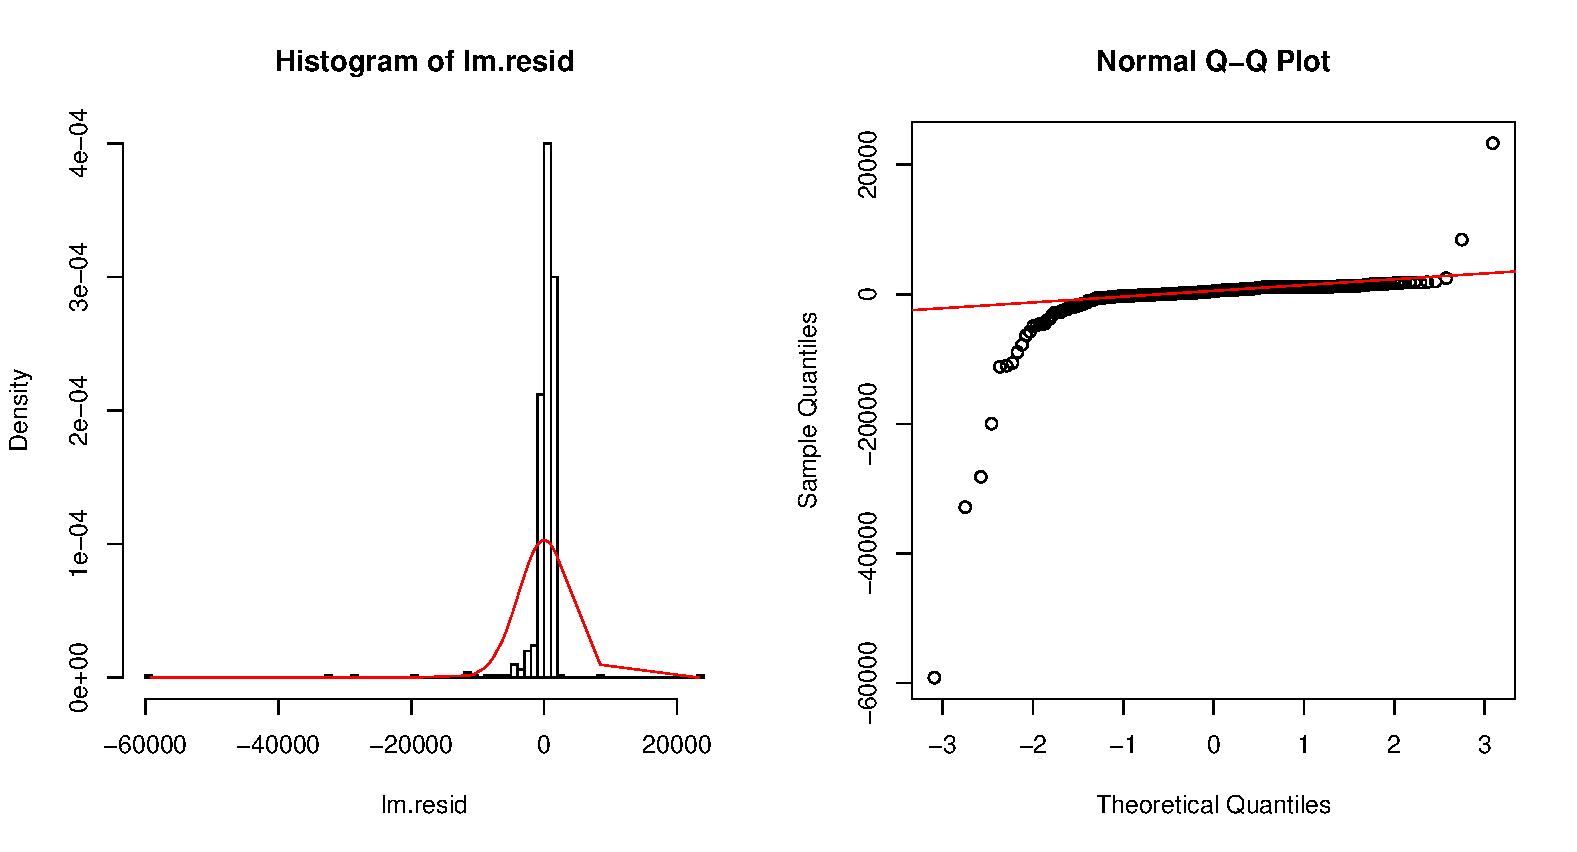
\includegraphics[scale=0.7]{imgs/residuals.pdf}
\end{figure}
\vspace{-0.8cm}
\begin{lstlisting}[language=bash,basicstyle=\tiny,tabsize=2,frame = single]
> shapiro.test(lm.resid)

	Shapiro-Wilk normality test

data:  lm.resid
W = 0.28981, p-value < 2.2e-16
\end{lstlisting}
\vspace{0.2cm}
Per approfondire, ho analizzato, la correlazione tra i predittori utilizzati, se
eventualmente i residui del modello fossero correlati con uno dei predittori, un
modello di regressione con tutti i predittori disponibili e un modello di
regressione lineare semplice. I risultati per\`o non sono stati comunque
soddisfacenti:
\vspace{0.2cm}
\begin{lstlisting}[language=bash,basicstyle=\tiny,tabsize=2,frame = single]
> cor(data$Rpeak, data$TotalCores)
[1] 0.7525282

> cor(data$Rpeak, lm.resid)
[1] 1.965037e-15

> cor(data$TotalCores, lm.resid)
[1] 8.458876e-16

> # approfondimento analisi dei residui: valutazione modello di regressione
> # lineare con tutti i fattori
> lm.1.resid = residuals(lm.1)
> shapiro.test(lm.1.resid)

	Shapiro-Wilk normality test

data:  lm.1.resid
W = 0.31715, p-value < 2.2e-16

> # approfondimento analisi dei residui: valutazione modello di regressione
> # lineare semplice
> lm.4.resid = residuals(lm.4)
> shapiro.test(lm.4.resid)

	Shapiro-Wilk normality test

data:  lm.4.resid
W = 0.27671, p-value < 2.2e-16
\end{lstlisting}
\vspace{0.2cm}
La mia ipotesi allora, dato che la distribuzione \`e comunque centrata in zero e
ricorda l'andamento di una Gaussiana, \`e stata che fosse a causa della presenza
di alcuni valori numerici eccessivamente elevati rispetto alla media. Dopo aver
rimosso questo primo sotto insieme di residui, ho notato che probabilmente fosse
necessario rimuovere una parte dei residui che causavano una forte deviazione
da una distribuzione Gaussiana. Cos\`i facendo ho ottenuto un modello certamente
migliore ma comunque non perfetto:
\clearpage
\begin{figure}[H]
	\vspace{-1cm}
	\begin{center}
		\hspace*{-1.5cm}
		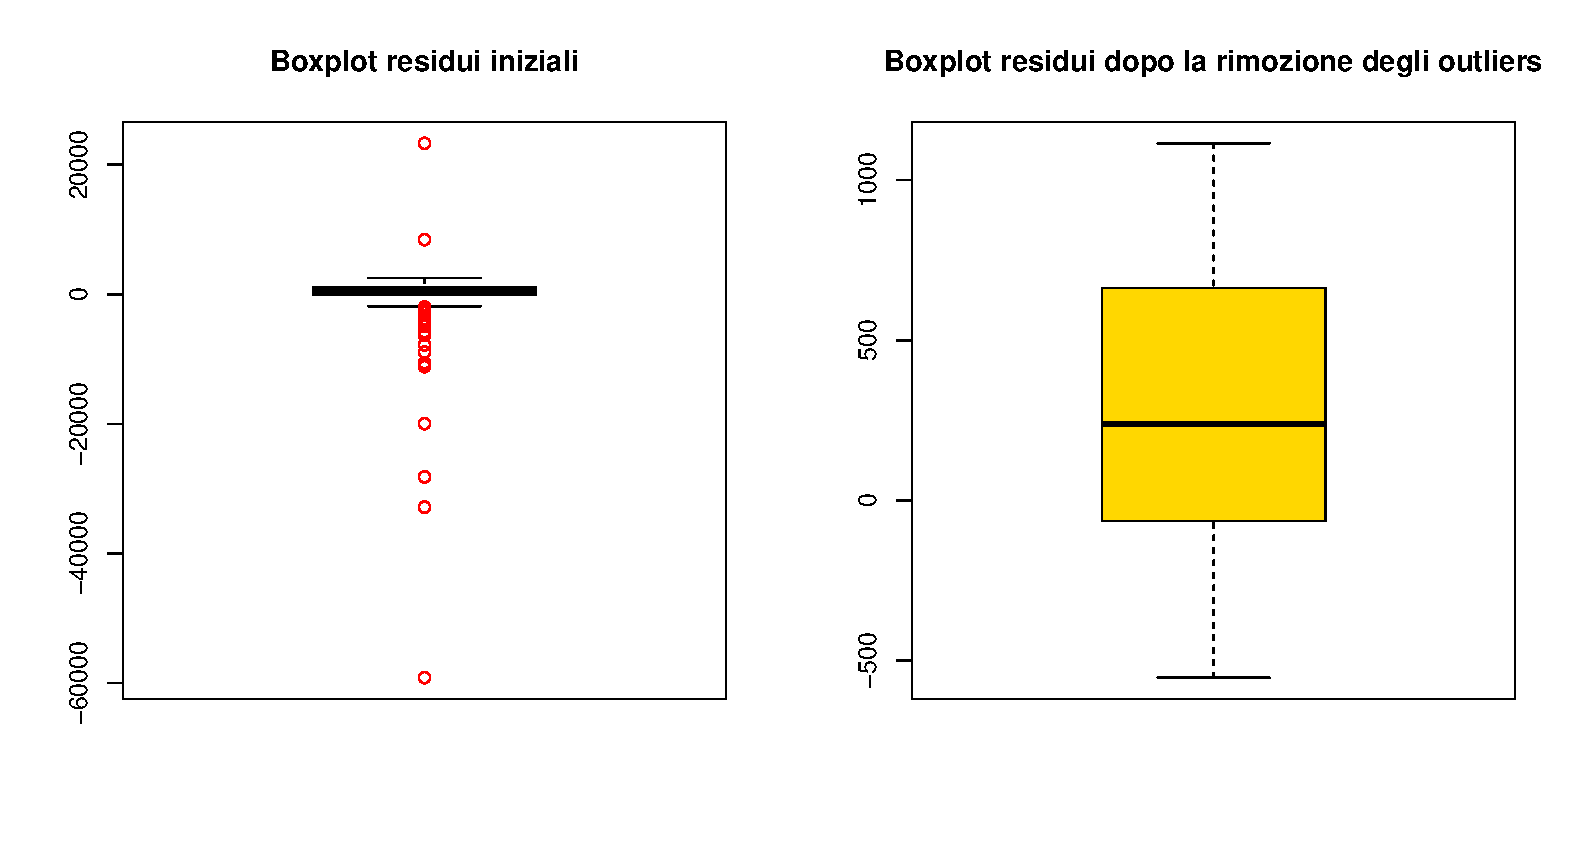
\includegraphics[scale=0.7]{imgs/residuals_boxplots.pdf}\\
		\vspace{-1.5cm}
		\hspace*{-1.5cm}
		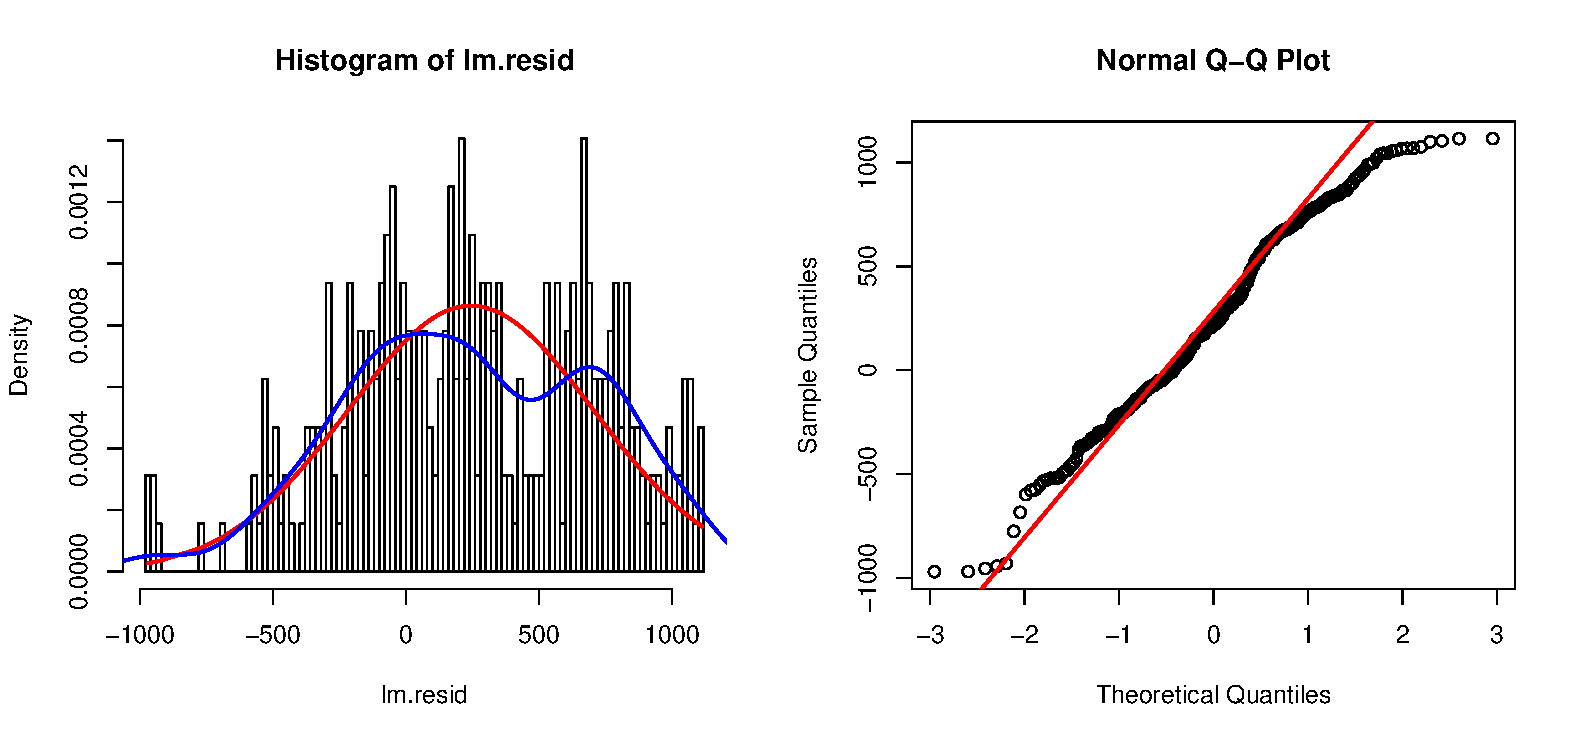
\includegraphics[scale=0.7]{imgs/residuals_2.pdf}
	\end{center}
\end{figure}
\vspace{-1cm}
\begin{lstlisting}[language=bash,basicstyle=\tiny,tabsize=2,frame = single]
> shapiro.test(lm.resid)

	Shapiro-Wilk normality test

data:  lm.resid
W = 0.97162, p-value = 8.588e-06
\end{lstlisting}
Da notare comunque la diminuzione di del valore del p-value di $10$ ordini di
grandezza.

\subsection{Modello di Regressione Esponenziale}
Non contento, nella speranza di riuscire ad ottenere un modello di regressione
con un valore di $\boldsymbol{R^2}$ leggermente minore, ma con una distribuzione
dei residui migliore, ho provato una analisi tramite modello di regressione
esponenziale.

\subsubsection{Analisi dei Residui}

\section{Conclusioni}

\end{document}
